\documentclass[11pt,a4paper]{article}

\usepackage{fullpage}
\usepackage{hyperref}
\usepackage{graphicx}
\usepackage{enumerate}
\usepackage{tikz}
\usepackage[bottom]{footmisc}
\usetikzlibrary{shapes, arrows, positioning, fit, backgrounds}
\usepackage{color}
\definecolor{pblue}{rgb}{0.13,0.13,1}
\usepackage{listings}
\lstset{language=Java,
		keywordstyle=\color{pblue},
		 breaklines=true,
		 basicstyle=\small,
		 tabsize=2
}
\usepackage{fancyhdr}
\pagestyle{fancy}
\fancyhf{}

\renewcommand{\headrulewidth}{0pt}
\renewcommand{\footrulewidth}{0pt}

\fancypagestyle{firstpagefooter} {
	\lfoot{\tiny{Version: 02.12.2017}}
	\cfoot{}
	\rfoot{\thepage}
	
}

\lfoot{Name: Simon Haefeli , Legi: 13-918-107}
\rfoot{\thepage}

\begin{document}

\title{Advanced Systems Lab Report\\ \normalsize{Autumn Semester 2017}}
\author{Name: Simon Haefeli\\Legi: 13-918-107}
\date{
	\vspace{4cm}
	\textbf{Grading} \\
	\vspace{0.5cm}
	\begin{tabular}{|c|c|}
		\hline  \textbf{Section} & \textbf{Points} \\
		\hline  1                &                 \\ 
		\hline  2                &                 \\ 
		\hline  3                &                 \\ 
		\hline  4                &                 \\ 
		\hline  5                &                 \\ 
		\hline  6                &                 \\ 
		\hline  7                &                 \\ 
		\hline \hline Total      &                 \\
		\hline 
	\end{tabular} 
}
\maketitle
\thispagestyle{firstpagefooter}

\newpage


\section{System Overview}
\subsection{Abstract}
This project consisted of designing, implementing and evaluating the performance of a key-value store network system. We added a so called middleware between the memtier benchmark clients and the memcached servers that was able to forward the requests and answers and do some processing for certain particular requests. In this report, we are first discussing the way the middleware has been implemented, analyze results of different experiments and finally modelling our system. 
\subsection{General design and implementation particularities}
Even though the general structure of the middleware was clearly defined, the components of the middlware asked for some important design choices. Here follow a small overview of the different implementation choices. 

\begin{center}
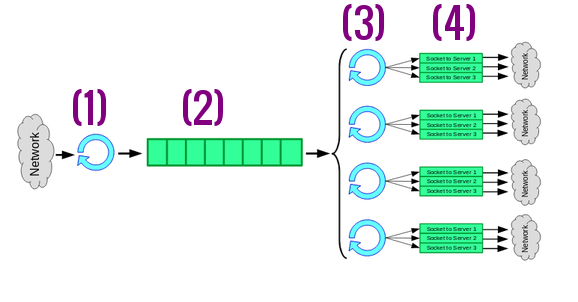
\includegraphics[scale=0.7]{baseIm.png}
\end{center}
\begin{enumerate}[ {(}1{)} ]
\item The net thread is the thread that accepts connections from the clients, and reads the incoming requests to put them in the request queue (2). The \textit{Java.nio} (non-blocking IO) package was used to achieve this purpose: A \textit{ServerSocketChannel} was used as a welcome socket to accept connections from the clients by creating for each client a \textit{SocketChannel}, and a \textit{Selector} was used to iterate over the the sockets (the connection sockets and the welcome socket) to find entering requests for the middleware or connection requests. Using the \textit{Java.nio} allows us not only to abstract the handling of a various number of connections, but also iterates over the client connections in an optimal way by using \textit{SelectionKeys}. 
\item The request queue is a java \textit{LinkedBlockingQueue}, which has the nice properties to be unbounded and beeing FCFS. Requests wait in this queue until a worker thread is free.   

\item The request queue and the worker threads are both managed by the java \textit{ThreadPoolExecutor}. The thread pool executor,which definition is: 
\begin{lstlisting}
	ThreadPoolExecutor(int corePoolSize, int maximumPoolSize, long keepAliveTime, TimeUnit unit, LinkedBlockingQueue workQueue)
\end{lstlisting} 
has a fixed number of worker threads by setting corePoolSize = maximumPoolSize. Putting a request into the queue or executing it, depending on the availability of the worker threads is beeing done by the same following instruction:
\begin{lstlisting}
	myThreadPoolExecutor.execute(Runnable command)
\end{lstlisting}
The \textit{ThreadPoolExecutor} will execute the command if a worker thread is available, or put it to the unbounded queue if not, which is exactly the expected behaviour.\footnote{https://docs.oracle.com/javase/7/docs/api/java/util/concurrent/ThreadPoolExecutor.html, part on "Queuing"}     
 
\item The connection sockets with the memcached servers are normal Java \textit{Socket}. Each worker thread opens a socket to each memcached server the first time it is beeing run and keeps it open until the middleware is stopped.  
\end{enumerate}

\subsection{Request handling}
We now want to look closer at the implementation of the middleware and how the pipeline looks like for a request beeing processed. The following flow chart illustrates this:
\\
\\\\
% Define block styles]
\tikzstyle{block} = [rectangle, draw, fill=blue!20, 
    text width=9em, text centered, rounded corners, minimum height=4em]
\tikzstyle{line} = [draw, -latex']
\tikzstyle{cloud} = [draw, ellipse,fill=red!20, node distance=3cm,
    minimum height=2em]   
\begin{tikzpicture}[node distance = 3cm, auto]
    % Place nodes
    \node [block] (RunMW) {\textbf{\underline{RunMW}} \\ \textit{main(): starts the mw}};
    \node [block, below=0.7cm of RunMW] (MyMiddleware) {\textbf{\underline{MyMiddleware}} \\ \textit{run(): reads the text from the socket and creates a prerequest}};
    \node [block, left=3cm of MyMiddleware, text width=8em] (Params) {\underline{Params} \\ inputs predefined parameters};
    \node [block, right=2cm of MyMiddleware] (PreRequest) {\textbf{\underline{PreRequest}} \\ \textit{PreRequest(): creates an object with the text and a starting time}};
    \node [block, below of=MyMiddleware] (QueueHandler) {\textbf{\underline{QueueHandler}} \\ \textit{putToQueue(): calls the threadPoolExecutor execute function on the Prerequest}};
    \node [block, left=3cm of QueueHandler, text width=11em] (StatisticsAggregator) {\textbf{\underline{StatisticsAggregator}} \\ \textit{run(): Gets statistics from different classes every time window, processes them and stores in the Statistics class}};
     \node [block, below of=StatisticsAggregator, text width=8em] (Statistics) {\underline{Statistics} \\ Contains the aggregated statistics};
      \node [block, below=1cm of QueueHandler] (RequestHandler) {\textbf{\underline{RequestHandler}} \\ \textit{run(): creates a Request to parse the PreRequest and calls the appropriate handling function}};
      \node [block, right=2cm of RequestHandler, text width=8em] (Request) {\textbf{\underline{Request}} \\ \textit{Request(): parses the text received from the client with the correct RequestType}};
      \node [block, above of=Request] (RequestType) {\underline{RequestType} \\ Contains the different request types};
      \node [cloud, below=0.8cm of RequestHandler] (HandleGet) {HandleGet()};
      \node [cloud, right=0.5cm of HandleGet] (HandleSet) {HandleSet()};
      \node [cloud, left=0.5cm of HandleGet] (HandleMGet) {HandleMGet()};
      
    % Draw edges
    \path [line] (RunMW) -- (MyMiddleware);
    \draw[>=latex,->] ([yshift= -5pt] PreRequest.west) -- ([yshift= -5pt] MyMiddleware.east);
    \draw[>=latex,<-] ([yshift= 5pt] PreRequest.west) -- ([yshift= 5pt] MyMiddleware.east);
  
    \path [line] (Params) -- (MyMiddleware);
    \path [line, dashed] (MyMiddleware) -- (StatisticsAggregator);
    \path [line, dashed] (QueueHandler) -- (StatisticsAggregator);
    \path [line, dashed] (RequestHandler) -- (StatisticsAggregator);
    \path [line] (StatisticsAggregator) -- (Statistics);
    \path [line] (MyMiddleware) -- (QueueHandler);
    \path [line] (QueueHandler) -- (RequestHandler);
    \draw[>=latex,->] ([yshift= 5pt] RequestHandler.east) -- ([yshift= 5pt] Request.west);
    \draw[>=latex,<-] ([yshift= -5pt] RequestHandler.east) -- ([yshift= -5pt] Request.west);
    \draw[>=latex,<-] ([xshift= 5pt] Request.north) -- ([xshift= 5pt] RequestType.south);
    \draw[>=latex,->] ([xshift= -5pt] Request.north) -- ([xshift= -5pt] RequestType.south);
    \path [line] (RequestHandler) -- (HandleMGet);
    \path [line] (RequestHandler) -- (HandleGet);
    \path [line] (RequestHandler) -- (HandleSet);
\end{tikzpicture}

\newpage

To make some correpondencies with the general structure of the middleware presented in section 1.2, we see that the \textit{MyMiddleware run()} function represents the net thread, the \textit{QueueHandler} class has a \textit{ThreadPoolExecutor} field that manages the request queue and the call of the worker thread, and that the \textit{RequestHandler run()} function represents one worker thread. We may also note that a PreRequest class is beeing created before putting the received message into the queue. This is to bind the message with a time, to be able to track the time a message spends in the queue. 
\\\\
At the end of the pipeline, the different requests are treated according to their type (get, set, or multi-get). In case of a set, the request is sent to all memcached servers sequentially, after what the worker thread waits for all the answers, also sequentially, as showed in the next line in the case of 3 memcached servers. 
\begin{lstlisting}
	1				send to server 1
	2				send to server 2
	3				send to server 3
	4				wait for answer 1 until received
	5				wait for answer 2 until received
	6				wait for answer 3 until received
	7				merge the answers and send back to client
\end{lstlisting}
The main drawback of this design is that if one of the server has a higher latency than the other ones, the worker thread might be waiting idle instead of starting to read the answers from the other servers. 
\\
In case of a get request, we simply forward the request to a given server. To decide which memcached server we send the request, we simply keep a static field in the \textit{RequestHandler} class which is shared accross the worker threads that keeps track of the last server to which we sent a get request. This variable is then beeing updated in a round-robin way. 
\\
In case of a multi-get, two cases are possible: In the non-sharded case, the request is simply beeing executed as a normal get. In the sharded case, the multi get is beeing splitted equally accross the different available memcached servers.   
\\\\
Finally, since we want the connections between the middleware and the servers to be open before running the experiments, we need to initialize these once for every worker thread. By defining the sockets in a \textit{ThreadLocal} in the \textit{RequestHandler} class, the initialization of the sockets will happen only the first time a worker thread is beeing called. That's why every thread is called once during the initialization phase of the middleware, by executing number of worker threads "init" requests, which are fake requests that don't need any special handling.\footnote{According to the javadoc of the ThreadPoolExecutor class, "When a new task is submitted in method execute(java.lang.Runnable), and fewer than corePoolSize threads are running, a new thread is created to handle the request, even if other worker threads are idle". And that's why it is enough to run corePoolSize number of requests to have them run all once and thus initialized their sockets.} 

\subsection{Statistics gathering}
Statistics have to be made in different classes accross the middleware, either a count (number of gets, number of sets,...), or an average (queue length, time in queue,...). These statistics are beeing stored in static atomic fields in the respective classes, that can be gotten from the \textit{StatisticsAggregator} class, which is a \textit{Runnable} called every second, the first time at initialization of the middleware. These statistics are then collected every given time window, averaged and stored in the \textit{Statistics} class. This process is beeing illustrated in the next figure:
\\
% Define block styles]
\tikzstyle{block} = [rectangle, draw, fill=green!20, 
    text width=36em, text centered, rounded corners, minimum height=4em]
\tikzstyle{line} = [draw, -latex'] 
\begin{tikzpicture}[node distance = 3cm, auto]
    % Place nodes
      \node [block, text width=36em] (StatisticsAggregator) {\textbf{\underline{StatisticsAggregator}} \\\begin{lstlisting}
	public void run(){
		int timesInQueue = Requesthandler.timesInQueue.getAndSet(0);
		int timesInQueueCount = Requesthandler.timesInQueueCount.getAndSet(0);
		Statistics.queueTimes.add(timesInQueue/timesInQueueCount);
	}
\end{lstlisting}};
    \node [block,text width=31em, below=6cm of StatisticsAggregator.west, anchor=west] (RequestHandler) {\textbf{\underline{RequestHandler}} \\\begin{lstlisting}
	public static AtomicInteger timesInQueue = 0;
	public static AtomicInteger timesInQueueCount = 0;
	public void handleRequest(request){
		ellapsedTime = System.nanoTime()-request.startTime;
		timesInQueue.getAndAdd(ellapsedTime);
		timesInQueueCount.getAndIncrement();
	}
\end{lstlisting}};
    \node [block, right=9cm of RequestHandler.north, anchor=north, text width = 10em] (Statistics) {\underline{Statistics} \\\begin{lstlisting}
	List<Integer> queueTimes;
\end{lstlisting}};
      
    % Draw edges
    \path [line] (StatisticsAggregator) -| (Statistics);
    \draw[>=latex,->] ([xshift= -5pt] RequestHandler.north) -- ([xshift= -5pt] StatisticsAggregator.south);
    \draw[>=latex,<-] ([xshift= 5pt] RequestHandler.north) -- ([xshift= 5pt] StatisticsAggregator.south);

\end{tikzpicture}
\\\\
The collected statistics in the \textit{Statistics} class are then beeing filtered, by removing the warm-up time (according to some experiments I made, the middlware needs around 10 seconds to get stable data) and the cool down time (1 second), and removing the zero values that are present before and after the significative values (zeros that occur because of the late start of a memtier client for example or an early stop). 
\\
Finally, when the middleware is shut down, the average and standart deviation of every statistic is beeing computed and printed to a file. Depending on the experiment, we sometimes also print all the values to construct histograms.
\newpage  
\section{Baseline without Middleware}
The goal of this experiment is to study how the system would perform without the middleware. This part is important to get a better idea of what the performance limitations of the memcached servers and the memtier benchmark clients are, so we can better judge of the impact of the middleware through the rest of the experiments. 

\subsection{One Server}

First, we want to analyze the performance evolution of the memcached server, and eventually find its upper-bound in terms of performance. To achieve this, we set up one single memcached server beeing queried by a various number of clients, for read-only and write-only workloads. More precisely, we are running experiments in the following configuration:
\begin{center}
	\scriptsize{
		\begin{tabular}{|l|c|}
			\hline Number of servers                & 1                        \\ 
			\hline Number of client machines        & 3                        \\ 
			\hline Instances of memtier per machine & 1                        \\ 
			\hline Threads per memtier instance     & 2                        \\
			\hline Virtual clients per thread       & [1..32]                  \\ 
			\hline Workload                         & Write-only and Read-only \\
			\hline 
		\end{tabular}
	} 
\end{center}

\subsubsection{Results and explanation}
For a read only workload, we obtain the following plots for the latency and the throughput, for one client machine (the plots are very similar than the ones of the other client machines):
\\
\begin{minipage}{0.5\linewidth}
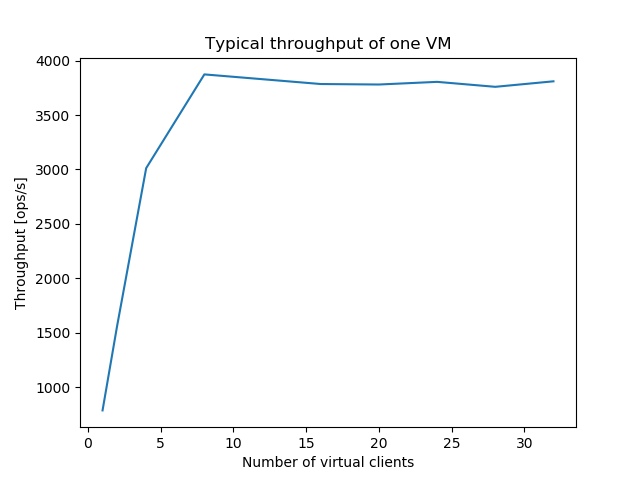
\includegraphics[width=\linewidth]{/home/simon/Documents/ETH/asl/asl-fall17-project/collectedStatFiles/Exp2/baseline1/readOneVMThroughput.png}
\end{minipage}
\hfill
\begin{minipage}{0.5\linewidth}
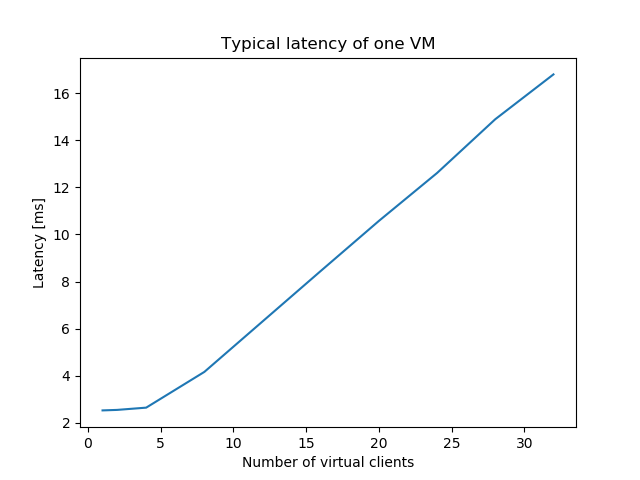
\includegraphics[width=\linewidth]{/home/simon/Documents/ETH/asl/asl-fall17-project/collectedStatFiles/Exp2/baseline1/readOneVMLatency.png}
\end{minipage}
\\\\
We notice that the maximum throughput is already obtained with 8 virtual clients per virtual machine and is then stable as we let the number of clients grow. This is, the memcached server starts to saturate when 3 VM with 2 threads and 8 virtual clients are querying a single server simultaneously. It is important to mention here that it is nearly impossible to over-saturate a server due to the way the memtier benchmark work: since we always run the clients with the default \textit{--pipeline=1} argument, every CPM\footnote{virtual client per memtier, see project description} will wait for an answer to come back before sending another request.
\\
For the latency, we clearly see that is inversely proportionnal to the througput (we distinguish three different slopes on both graphs). In the phase When the number of virtual clients grows at a constant rate (number of virtual clients getting bigger than 8), the throughput also gets constant. The reason why the throughput doesn't drop but stays at approximately 4000 operations/second is because the higher latency is compensated by a higher number of virtual clients to keep the throughput constant. 
\\\\
For a write-only workload, we obtain the following results:
\\
\begin{minipage}{0.5\linewidth}
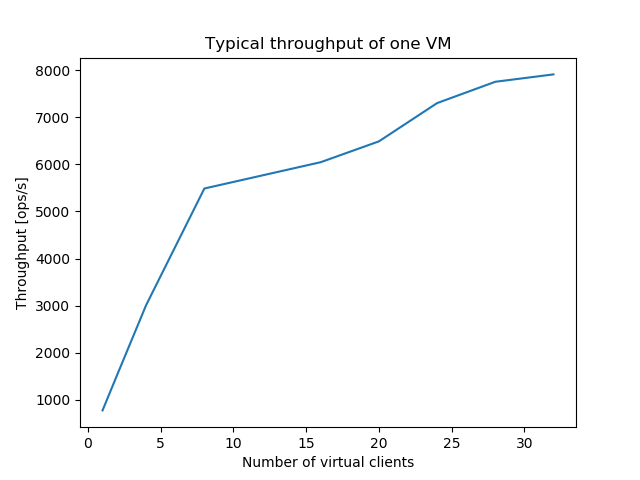
\includegraphics[width=\linewidth]{/home/simon/Documents/ETH/asl/asl-fall17-project/collectedStatFiles/Exp2/baseline1/writeOneVMThroughput.png}
\end{minipage}
\hfill
\begin{minipage}{0.5\linewidth}
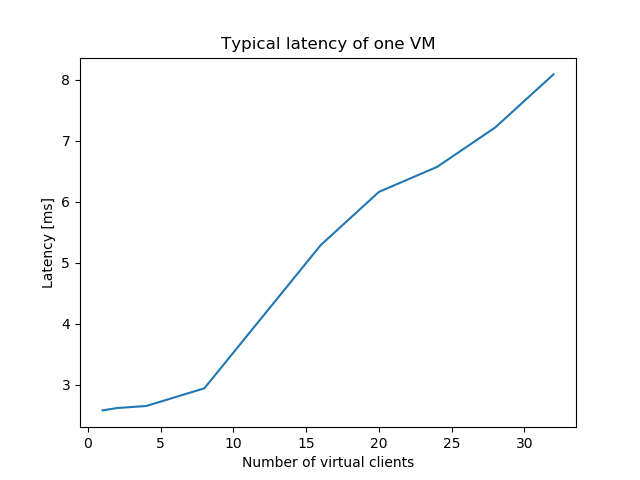
\includegraphics[width=\linewidth]{/home/simon/Documents/ETH/asl/asl-fall17-project/collectedStatFiles/Exp2/baseline1/writeOneVMLatency.png}
\end{minipage}
\\\\\\
For this workload, we note that we barely reach a saturated memcached server with 32 virtual clients, even if there is a clear drop in the growth of the throughput at 8 virtual clients. For write-only, the same observations apply as for the read-only workload. 
\\\\
However, we note a maximum throughput twice as high for sets than for gets, with a maximum latency twice as small. The differnce size of the messages beeing sent back and forth between the clients and the servers may not be the main factor, since for a get the messages are: 
\begin{lstlisting}
	request: get memtier-9999, 		answer: value memtier-9999 XXXXXX
\end{lstlisting}
and for the set they are:
\begin{lstlisting}
	request: set memtier-9999  0 10000 1024 XXXXX,	answer:  STORED
\end{lstlisting}
which are quite the same length. This implies that memcached is either storing values faster than getting values, either send the \textit{STORED} message back before starting the write operation, either having poorer performance than memtier benchmark when writting big messages to the connection sockets, or a combination of these factors. For this report, we will just keep in mind that the achieved throughput is higher with a write-only workload.
   
\subsection{Two Servers}

Now we are increasing the number of servers and putting a single client machine with a single thread to measure the see the performance limitations of the memtier clients with the following configurations:

\begin{center}
	\scriptsize{
		\begin{tabular}{|l|c|}
			\hline Number of servers                & 2                        \\ 
			\hline Number of client machines        & 1                        \\ 
			\hline Instances of memtier per machine & 2                        \\ 
			\hline Threads per memtier instance     & 1                        \\
			\hline Virtual clients per thread       & [1..32]                  \\ 
			\hline Workload                         & Write-only and Read-only \\
			\hline 
		\end{tabular}
	} 
\end{center}

\subsubsection{Results and explanation}
For a read-only workload, we obtain the following plots:
\\
\begin{minipage}{0.5\linewidth}
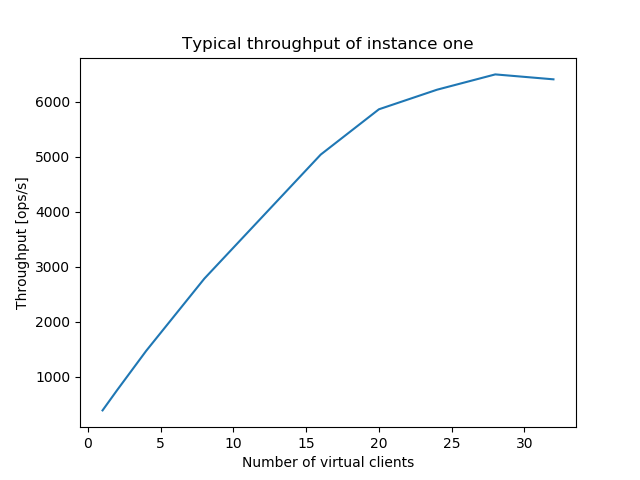
\includegraphics[width=\linewidth]{/home/simon/Documents/ETH/asl/asl-fall17-project/collectedStatFiles/Exp2/baseline2/readInst1Throughput.png}
\end{minipage}
\hfill
\begin{minipage}{0.5\linewidth}
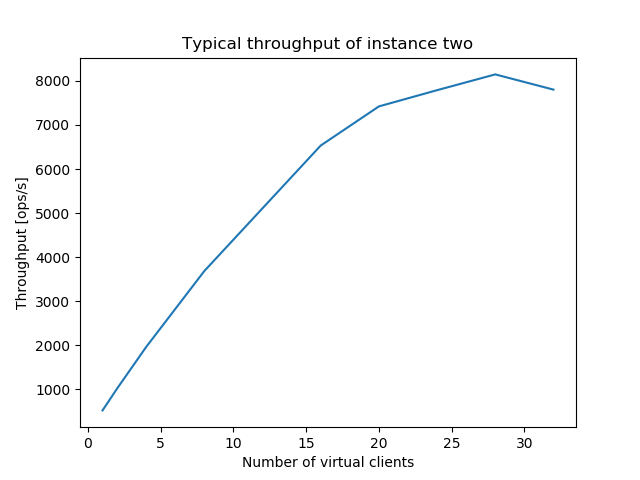
\includegraphics[width=\linewidth]{/home/simon/Documents/ETH/asl/asl-fall17-project/collectedStatFiles/Exp2/baseline2/readInst2Throughput.png}
\end{minipage}
\\\\
Remember that the client machine has two instances each connected to a different memcached server. It is important to notice at this point that the maximal throughput achieved by the two instances are not equal. As shown on the next figures, this is because the latency is higher for one of the two servers, which may be because of their geographic location (The server located further away from the client machine results in a higher latency).
\begin{minipage}{0.5\linewidth}
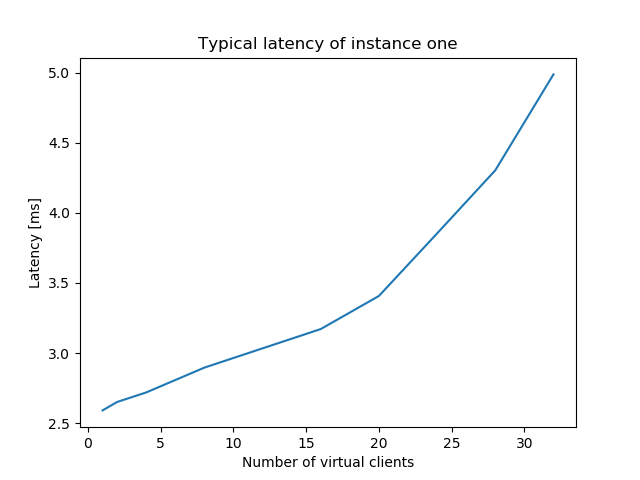
\includegraphics[width=\linewidth]{/home/simon/Documents/ETH/asl/asl-fall17-project/collectedStatFiles/Exp2/baseline2/readInst1Latency.png}
\end{minipage}
\hfill
\begin{minipage}{0.5\linewidth}
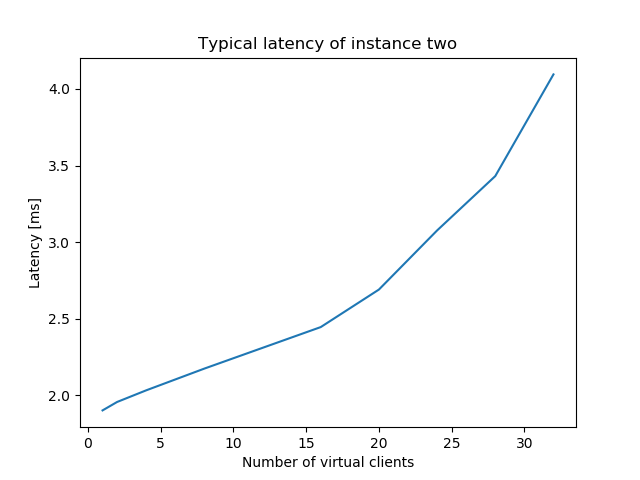
\includegraphics[width=\linewidth]{/home/simon/Documents/ETH/asl/asl-fall17-project/collectedStatFiles/Exp2/baseline2/readInst2Latency.png}
\end{minipage}
\\\\
For a write-only workload, we obtain for the server with higher througput similar plots for throughput and latency than for a read-only workload:
\\
\begin{minipage}{0.5\linewidth}
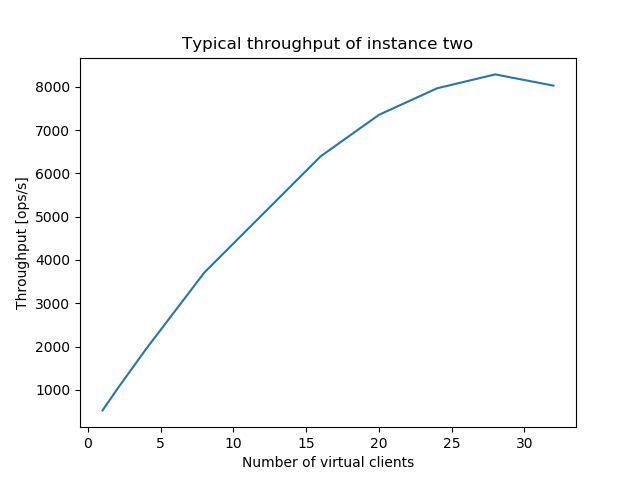
\includegraphics[width=\linewidth]{/home/simon/Documents/ETH/asl/asl-fall17-project/collectedStatFiles/Exp2/baseline2/writeInst2Throughput.png}
\end{minipage}
\hfill
\begin{minipage}{0.5\linewidth}
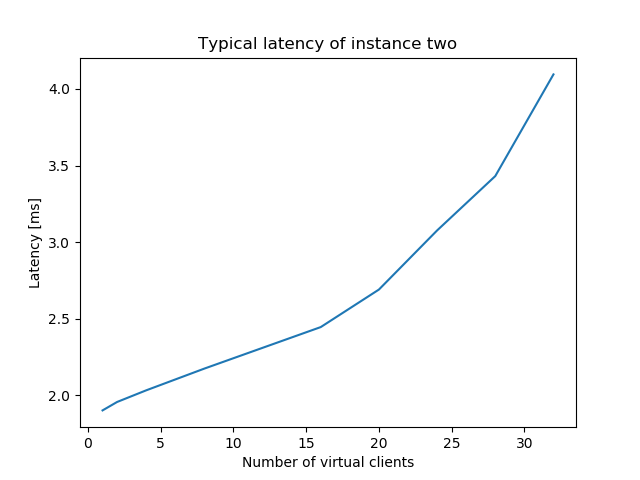
\includegraphics[width=\linewidth]{/home/simon/Documents/ETH/asl/asl-fall17-project/collectedStatFiles/Exp2/baseline2/writeInst2Latency.png}
\end{minipage}
\\
\\
We see that the system starts to saturate for the two workloads when reaching 28 virtual clients per thread, with a maximum throughput of around 8000 operations per second for the instance with more higher throughput.  
We also note that contrary to the last experiment with a single server, the throughput for write and read are similar. This proves for the last experiment, that the memcached server saturates under a high workload, but tends to be more scalable for get-only operations. On the other hand, a single client machine cannot produce a higher throughput than 8000 operations per second, for read and for write.   
\subsection{Summary}


Based on the experiments, we are now able to fill the table with the maximal throughputs for different configurations. For one memcached server, we use the results of one single client machine (which are representative of the results of the other client machines). For a single memtier client, we use the results of both instances to give a lower and upper bound (separated by a "/"). 

\begin{center}
	{Maximum throughput meaasured on one VM}
	\begin{tabular}{|l|p{2cm}|p{2cm}|p{4cm}|}
		\hline                        & Read-only workload & Write-only workload & Configuration gives max. throughput \\ 
		\hline One memcached server   &4102                    &8430                     &8 VC for read-only, 32  VC for write-only                                     \\ 
		\hline One load generating VM &6498/8146                    &6558/8287                     &28 VC                                     \\ 
		\hline 
	\end{tabular}
\end{center}
As explained in the previous sections, the key take-aways this experiment are the following:

\begin{itemize}
\item The achieved throughput by the memtier clients and even instances may be vary: because of the geographic positions of the clients or other factors. 
\item The memcached servers saturate faster for a read-only workload. For a write-only workload, the throughput can be twice as high and is limited by the performance of the memtier clients. 
\end{itemize}
\newpage

\section{Baseline with Middleware}

In this set of experiments we want to take a closer look on the effect of the middleware on the system. For this purpose, we are running experiments with different workloads, a different number of worker threads in the middleware, and one or two middlewares. This will show us in what way the middleware influences the results found during experiment two. 


\subsection{One Middleware}

We start the experiment by connecting a single client machine to the middleware and one memcached server, for different workloads and number of worker threads: 

\begin{center}
	\scriptsize{
		\begin{tabular}{|l|c|}
			\hline Number of servers                & 1                        \\ 
			\hline Number of client machines        & 1                        \\ 
			\hline Instances of memtier per machine & 1                        \\ 
			\hline Threads per memtier instance     & 2                        \\
			\hline Virtual clients per thread       & [1..32]                  \\ 
			\hline Workload                         & Write-only and Read-only \\
			\hline Number of middlewares            & 1                        \\
			\hline Worker threads per middleware    & [8..64]                  \\
			\hline 
		\end{tabular}
	} 
\end{center}

\subsubsection{Results and explanation}


Provide a detailed analysis of the results (e.g., bottleneck analysis, component utilizations, average queue lengths, system saturation). Add any additional figures and experiments that help you illustrate your point and support your claims.

\subsection{Two Middlewares}

Connect one load generator machine (two instances of memtier with CT=1) to two middlewares and use 1 memcached server. Run a read-only and a write-only workload with increasing number of clients (between 2 and 64) and measure response time \emph{both at the client and at the middleware}, and plot the throughput and response time as measured in the middleware.

Repeat this experiment for different number of worker threads inside the middleware: 8, 16, 32, 64.

If in your experiment the middleware is not the bottleneck, repeat the experiment that reaches the highest throughput but using two load generator VMs (each with 2x memtier CT=1) instead of one. Otherwise, explain how you know that the middlewares are the limiting factor in terms of throughput.

\begin{center}
	\scriptsize{
		\begin{tabular}{|l|c|}
			\hline Number of servers                & 1                        \\ 
			\hline Number of client machines        & 1                        \\ 
			\hline Instances of memtier per machine & 2                        \\ 
			\hline Threads per memtier instance     & 1                        \\
			\hline Virtual clients per thread       & [1..32]                  \\ 
			\hline Workload                         & Write-only and Read-only \\
			\hline Multi-Get behavior               & N/A                      \\
			\hline Multi-Get size                   & N/A                      \\
			\hline Number of middlewares            & 2                        \\
			\hline Worker threads per middleware    & [8..64]                  \\
			\hline Repetitions                      & 3 or more (at least 1 minute each)                \\ 
			\hline 
		\end{tabular}
	} 
\end{center}

\subsubsection{Explanation}

Provide a detailed analysis of the results (e.g., bottleneck analysis, component utilizations, average queue lengths, system saturation). Add any additional figures and experiments that help you illustrate your point and support your claims.

\subsection{Summary}

Based on the experiments above, fill out the following table. For both of them use the numbers from a single experiment to fill out all lines. Miss rate represents the percentage of GET requests that return no data. Time in the queue refers to the time spent in the queue between the net-thread and the worker threads.


\begin{center}
	{Maximum throughput for one middleware.}
	\begin{tabular}{|l|p{2cm}|p{2cm}|p{2cm}|p{2cm}|}
		\hline                                & Throughput & Response time & Average time in queue & Miss rate \\ 
		\hline Reads: Measured on middleware  &            &               &                       &           \\ 
		\hline Reads: Measured on clients     &            &               & n/a                   &           \\ 
		\hline Writes: Measured on middleware &            &               &                       & n/a       \\ 
		\hline Writes: Measured on clients    &            &               & n/a                   & n/a       \\ 
		\hline 
	\end{tabular}
\end{center}

\begin{center}
	{Maximum throughput for two middlewares.}
	\begin{tabular}{|l|p{2cm}|p{2cm}|p{2cm}|p{2cm}|}
		\hline                                & Throughput & Response time & Average time in queue & Miss rate \\ 
		\hline Reads: Measured on middleware  &            &               &                       &           \\ 
		\hline Reads: Measured on clients     &            &               & n/a                   &           \\ 
		\hline Writes: Measured on middleware &            &               &                       & n/a       \\ 
		\hline Writes: Measured on clients    &            &               & n/a                   & n/a       \\ 
		\hline 
	\end{tabular}
\end{center}

Based on the data provided in these tables, write at least two paragraphs summarizing your findings about the performance of the middleware in the baseline experiments.

\section{Throughput for Writes (90 pts)}

\subsection{Full System}

Connect three load generating VMs to two middlewares and three memchached servers. Run a write-only experiment. 
You need to plot throughput and response time measured on the middleware as a function of number of clients. The measurements have to be performed for 8, 16, 32 and 64 worker threads inside each middleware.

\begin{center}
	\scriptsize{
		\begin{tabular}{|l|c|}
			\hline Number of servers                & 3          \\ 
			\hline Number of client machines        & 3          \\ 
			\hline Instances of memtier per machine & 2          \\ 
			\hline Threads per memtier instance     & 1          \\
			\hline Virtual clients per thread       & [1..32]    \\ 
			\hline Workload                         & Write-only \\
			\hline Multi-Get behavior               & N/A        \\
			\hline Multi-Get size                   & N/A        \\
			\hline Number of middlewares            & 2          \\
			\hline Worker threads per middleware    & [8..64]    \\
			\hline Repetitions                      & 3 or more (at least 1 minute each)  \\ 
			\hline 
		\end{tabular}
	} 
\end{center}

\subsubsection{Explanation}

Provide a detailed analysis of the results (e.g., bottleneck analysis, component utilizations, average queue lengths, system saturation). Add any additional figures and experiments that help you illustrate your point and support your claims.

\subsection{Summary}

Based on the experiments above, fill out the following table with the data corresponding to the maximum throughput point for all four worker-thread scenarios.

\begin{center}
	{Maximum throughput for the full system}
	\begin{tabular}{|l|p{1.5cm}|p{1.5cm}|p{1.5cm}|p{1.5cm}|}
		\hline                                            & WT=8 & WT=16 & WT=32 & WT=64 \\ 
		\hline Throughput (Middleware)                    &      &       &       &       \\ 
		\hline Throughput (Derived from MW response time) &      &       &       &       \\ 
		\hline Throughput (Client)                        &      &       &       &       \\ 
		\hline Average time in queue                      &      &       &       &       \\ 
		\hline Average length of queue                    &      &       &       &       \\ 
		\hline Average time waiting for memcached         &      &       &       &       \\ 
		\hline 
	\end{tabular}
\end{center}

Based on the data provided in these tables, draw conclusions on the state of your system for a variable number of worker threads.

\section{Gets and Multi-gets (90 pts)}

For this set of experiments you will use three load generating machines, two middlewares and three memcached servers. Each memtier instance should have 2 virtual clients in total and the number of middleware worker threads is 64, or the one that provides the highest throughput in your system (whichever number of threads is smaller).

For multi-GET workloads, memtier will generate a mixture of SETs, GETs, and multi-GETs. Memtier only allows to specify the maximum number of keys in a multi-GET request. Therefore, be aware that requests can also contain fewer keys than the provided value. It is recommended to record the average size of the multi-GETs. You will have to measure response time on the client as a function of multi-get size, with and without sharding on the middlewares.

\subsection{Sharded Case}

Run multi-gets with 1, 3, 6 and 9 keys (memtier configuration) with sharding enabled (multi-gets are broken up into smaller multi-gets and spread across servers). Plot average response time as measured on the client, as well as the 25th, 50th, 75th, 90th and 99th percentiles.

\begin{center}
	\scriptsize{
		\begin{tabular}{|l|c|}
			\hline Number of servers                & 3                       \\ 
			\hline Number of client machines        & 3                       \\ 
			\hline Instances of memtier per machine & 2                       \\ 
			\hline Threads per memtier instance     & 1                       \\
			\hline Virtual clients per thread       & 2     		            \\ 
			\hline Workload                         & memtier-default             \\
			\hline Multi-Get behavior               & Sharded                 \\
			\hline Multi-Get size                   & [1..9]                  \\
			\hline Number of middlewares            & 2                       \\
			\hline Worker threads per middleware    & max. throughput config. \\
			\hline Repetitions                      & 3 or more (at least 1 minute each)               \\ 
			\hline 
		\end{tabular}
	} 
\end{center}

\subsubsection{Explanation}

Provide a detailed analysis of the results (e.g., bottleneck analysis, component utilizations, average queue lengths, system saturation). Add any additional figures and experiments that help you illustrate your point and support your claims.

\subsection{Non-sharded Case}

Run multi-gets with 1, 3, 6 and 9 keys (memtier configuration) with sharding disabled. Plot average response time as measured on the client, as well as the 25th, 50th, 75th, 90th and 99th percentiles.

\begin{center}
	\scriptsize{
		\begin{tabular}{|l|c|}
			\hline Number of servers                & 3                       \\ 
			\hline Number of client machines        & 3                       \\ 
			\hline Instances of memtier per machine & 2                       \\ 
			\hline Threads per memtier instance     & 1                       \\
			\hline Virtual clients per thread       & 2                		 \\ 
			\hline Workload                         & memtier-default             \\
			\hline Multi-Get behavior               & Non-Sharded             \\
			\hline Multi-Get size                   & [1..9]                  \\
			\hline Number of middlewares            & 2                       \\
			\hline Worker threads per middleware    & max. throughput config. \\
			\hline Repetitions                      & 3 or more (at least 1 minute each)               \\ 
			\hline 
		\end{tabular}
	} 
\end{center}

\subsubsection{Explanation}

Provide a detailed analysis of the results (e.g., bottleneck analysis, component utilizations, average queue lengths, system saturation). Add any additional figures and experiments that help you illustrate your point and support your claims.

\subsection{Histogram}

For the case with 6 keys inside the multi-get, display four histograms representing the sharded and non-sharded response time distribution, both as measured on the client, and inside the middleware. Choose the bucket size in the same way for all four, and such that there are at least 10 buckets on each of the graphs.

\subsection{Summary}

Provide a detailed comparison of the sharded and non-shareded modes. For which multi-GET size is sharding the preferred option? Provide a detailed analysis of your system. Add any additional figures and experiments that help you illustrate your point and support your claims.

\section{2K Analysis (90 pts)}

For 3 client machines (with 64 total virtual clients per client VM) measure the throughput and response time of your system in a 2k experiment with repetitions. All GET operations have a single key. Investigate the following parameters:

\begin{itemize}
		
	\item Memcached servers: 2 and 3
	\item Middlewares: 1 and 2
	\item Worker threads per MW: 8 and 32
	      	      
\end{itemize}

Repeat the experiment for (a)~a write-only, (b)~a read-only, and (c)~a 50-50-read-write workload.
For each of the three workloads, what is the impact of these parameters on throughput, respectively response time?

\begin{center}
	\scriptsize{
		\begin{tabular}{|l|c|}
			\hline Number of servers                & 2 and 3                                     \\ 
			\hline Number of client machines        & 3                                           \\ 
			\hline Instances of memtier per machine & 2                                           \\ 
			\hline Threads per memtier instance     & 1                                           \\
			\hline Virtual clients per thread       & 32                                     \\ 
			\hline Workload                         & Write-only, Read-only, and 50-50-read-write \\
			\hline Multi-Get behavior               & N/A                                         \\
			\hline Multi-Get size                   & N/A                                         \\
			\hline Number of middlewares            & 1 and 2                                     \\
			\hline Worker threads per middleware    & 8 and 32                                    \\
			\hline Repetitions                      & 3 or more (at least 1 minute each)                                   \\ 
			\hline 
		\end{tabular}
	} 
\end{center}

\section{Queuing Model (90 pts)}

Note that for queuing models it is enough to use the experimental results from the previous sections. It is, however, possible that the numbers you need are not only the ones in the figures we asked for, but also the internal measurements that you have obtained through instrumentation of your middleware.

\subsection{M/M/1}

Build queuing model based on Section 4 (write-only throughput) for each worker-thread configuration of the middleware. Use one M/M/1 queue to model your entire system. Motivate your choice of input parameters to the model. Explain for which experiments the predictions of the model match and for which they do not.

\subsection{M/M/m}

Build an M/M/m model based on Section 4, where each middleware worker thread is represented as one service.  Motivate your choice of input parameters to the model. Explain for which experiments the predictions of the model match and for which they do not.

\subsection{Network of Queues}

Based on Section 3, build a network of queues which simulates your system. Motivate the design of your network of queues and relate it wherever possible to a component of your system. Motivate your choice of input parameters for the different queues inside the network. Perform a detailed analysis of the utilization of each component and clearly state what the bottleneck of your system is. Explain for which experiments the predictions of the model match and for which they do not.

\end{document}
\grid
\grid
